\documentclass[master=cws,masteroption=gs]{kulemt}

\setup{title={Automatisch uitrol van SQL systemen en vergelijking van beschikbaarheid},
  author={Thomas Uyttendaele},
  promotor={Prof.\,dr.\,ir.\ Wouter Joosen},
  assessor={Ir.},
  assistant={Ir.\ B. Vanbrabant}}
% De volgende \setup mag verwijderd worden als geen fiche gewenst is.
\setup{filingcard,
  translatedtitle={Automatisch uitrol van SQL systemen en vergelijking van beschikbaarheid},
  udc=621.3,
  shortabstract={Hier komt een heel bondig abstract van hooguit 500
      woorden. \LaTeX\ commando's mogen hier gebruikt worden. Blanco lijnen
   (of het commando \texttt{\string\pa r}) zijn wel niet
   toegelaten!
  \endgraf \lipsum[2]}}
% Verwijder de "%" op de volgende lijn als je de kaft wil afdrukken
%\setup{coverpageonly}
% Verwijder de "%" op de volgende lijn als je enkel de eerste pagina's wil
% afdrukken en de rest bv. via Word aanmaken.
%\setup{frontpagesonly}

% Kies de fonts voor de gewone tekst, bv. Latin Modern
\setup{font=lm}

% Hier kun je dan nog andere pakketten laden of eigen definities voorzien

% Tenslotte wordt hyperref gebruikt voor pdf bestanden.
% Dit mag verwijderd worden voor de af te drukken versie.
\usepackage[pdfusetitle,colorlinks,plainpages=false]{hyperref}
\usepackage[dutch]{babel}
\usepackage{lipsum} % for dummy text only
\usepackage{todonotes}
\usepackage{csquotes}
\usepackage[backend=bibtex]{biblatex}
\usepackage[acronym]{glossaries}
\newglossaryentry{eventualconsistency}{
	name=eventuele consistentie,
	description= aaa
}

\newglossaryentry{rangequery}{
	name=range query,
	plural= range queries,
	description= Het opvragen van een set van records met behulp van een enkele query
}

\newglossaryentry{base}{
	name=BASE,
	description= aaa
}
\newglossaryentry{acid}{
	name=ACID,
	description= aaa
}

\newglossaryentry{nosql}{
	name=NoSQL,
	description= aaa
}

\newglossaryentry{horizontaalschaalbaar}{
	name=horizontaal schaalbaar,
	description= aaa
}

\newglossaryentry{yum}{
	name=yum,
	description= aaa
}

\newglossaryentry{apt-get}{
	name=apt-get,
	description= aaa
}

\newglossaryentry{CAP}{
	name=CAP,
	description= aaa
}

\newglossaryentry{IMP}{
	name=IMP,
	description= aaa
}

\newglossaryentry{DBMS}{
	name=DBMS,
	plural= DBMS's,
	description= aaa
}

\newglossaryentry{HDFS}{
	name=HDFS,
	description= Hadoop Distributed File System
}

\newglossaryentry{eventsupport}{
	name=event support,
	description= a
}

\makeglossaries
\bibliography{overige/referenties}
%%%%%%%
% Om wat tekst te genereren wordt hier het lipsum pakket gebruikt.
% Bij een echte masterproef heb je dit natuurlijk nooit nodig!
\IfFileExists{lipsum.sty}%
 {\usepackage{lipsum}\setlipsumdefault{11-13}}%
 {\newcommand{\lipsum}[1][11-13]{\par Hier komt wat tekst: lipsum ##1.\par}}
%%%%%%%

%\includeonly{hfdst-n}
\begin{document}

\begin{preface}
\todo{Voorwoord schrijven}
\lipsum
  
\end{preface}

\tableofcontents*
\listoftodos
\begin{abstract}
\todo{Abstract schrijven}

  In dit \texttt{abstract} environment wordt een al dan niet uitgebreide
  samenvatting van het werk gegeven. De bedoeling is wel dat dit tot
  1~bladzijde beperkt blijft.
  \lipsum
\end{abstract}

% Een lijst van figuren en tabellen is optioneel
%\listoffigures
%\listoftables
% Bij een beperkt aantal figuren en tabellen gebruik je liever het volgende:
\listoffiguresandtables
% De lijst van symbolen is eveneens optioneel.
% Deze lijst moet wel manueel aangemaakt worden, bv. als volgt:
\chapter{Lijst van afkortingen en symbolen}
\section*{Afkortingen}
\begin{flushleft}
  \renewcommand{\arraystretch}{1.1}
  \begin{tabularx}{\textwidth}{@{}p{12mm}X@{}}
    IMP   & Infrastructure Management Platform \\
    DBMS   & Databasemanagementsysteem \\
  \end{tabularx}
\end{flushleft}
\section*{Symbolen}
\begin{flushleft}
  \renewcommand{\arraystretch}{1.1}
  \begin{tabularx}{\textwidth}{@{}p{12mm}X@{}}
    42    & aaa \\
  \end{tabularx}
\end{flushleft}

% Nu begint de eigenlijke tekst
\mainmatter

\chapter{Inleiding}
\label{inleiding}
In dit hoofdstuk wordt het werk ingeleid. Het doel wordt gedefinieerd en er
wordt uitgelegd wat de te volgen weg is (beter bekend als de rode draad).

\todo{Schrijf inleiding}

%%% Local Variables: 
%%% mode: latex
%%% TeX-master: "masterproef"
%%% End: 

\chapter{Probleem- en doelstelling}

\section{Probleemstelling}
Sinds het begin van WEB 2.0 is het gebruik van het internet veranderd, van een statisch tot een dynamische omgeving waar iedereen een persoonlijke en individuele ervaring heeft. Samen met deze evolutie is ook het type, de hoeveelheid en het gebruik van data en de opslag ervan veranderd. 

\paragraph{}
Deze verandering kan allereerst toegeschreven worden aan de toename in het aantal website, daarnaast is ook de content van een webpagina veranderd, geen statische pagina's met enkel tekst maar ook afbeeldingen en (korte) videofragmenten zijn aanwezig. Deze content wordt ook niet meer enkel door de websitebeheerder online geplaatst maar de gebruikers kunnen zelf hun data invoegen en krijgen gepersonaliseerde en dynamische pagina's te zien. 
Tenslotte is ook de toename in het aantal gebruikers, op 30 juni 2012 waren er meer als 2.4 miljard gebruikers van het internet, een toename van meer als 500\% op 12 jaar tijd.  
\cite{WorldInternetStatics}

\paragraph{}
Al deze veranderingen hebben ook hun doorslag op de achterliggende infrastructuur. Waar kleinere en statische websites nog konden gehost worden op een enkele server, is dit niet meer het geval voor hedendaagse (populaire) websites. 
Een onderdeel van deze web applicaties is de databases waarin de vereiste data kan in worden opgeslagen worden en later opgevraagd worden. Veel van deze databases zijn ontworpen naar het systeem van de relationele databases, uitgewerkt naar Codd \cite{Codd:1970:RMD:362384.362685}.

Voor talrijke van de huidige applicaties is de voorwaarden voor dataopslag verschillend met deze van de jaren 70. Enkele systemen hebben geen nood meer aan onmiddellijke consistentie maar hebben genoeg aan \gls{eventualconsistency}. Onder andere omwille van deze reden is er een stroming van nieuwe database systemen gekomen genaamd \gls{nosql}. Onder deze noemer vallen vele systemen, elk eigen in hun soort en aangepast aan bepaalde manieren van dataopslag en de daarvoor nodige vereisten, een belangrijk element is het \gls{horizontaalschaalbaar} zijn van deze systemen. Met andere woorden, deze databases zijn ontworpen om de data over meerdere systemen te verspreiden om de load te verspreiden. 

\paragraph{}
\Gls{horizontaalschaalbaar} brengt verschillende voordelen mee, maar zorgt ook voor 2 problemen die in deze thesis zullen aanbod komen, namelijke de uitrol en daarnaast wat de implicaties zijn van een gedistribueerd datasysteem. 

\subsection{Uitrollen van gedistribueerde databases}
Voor geavanceerde toepassingen is het gebruik van gespecialiseerde en/of gedistribueerde databases een noodzaak. Maar de tijdsduur van de beslissing dat dit het geval is tot een werkende omgeving hebben, is niet te onderschatten en dit omwille van verschillende componenten. 

\paragraph{}Een eerste stap die doorlopen wordt, is het opzoeken van de nodige informatie over de verschillende databases, nu bestaan er al verschillende websites en papers waar informatie opgezocht kan worden, maar een consistente test bestaat niet. Een voorbeeld van een vergelijkingswebsite is bijvoorbeeld vsChart \cite{vsChart}, ook verschillende papers brengen vergelijkingen naar voor in onder andere performantie en de verschillende data modellen. Maar in de meeste gevallen blijft het aangeraden om de informatie op te zoeken op de website van de software zelf, deze evolueert snel en informatie van een jaar oud kan al verouderd zijn en zo incorrect. 

Al deze informatie zou de ontwikkelaar een mogelijkheid geven om de verschillende systemen te kunnen vergelijken en een keuze te maken met welke database hij verder wenst te gaan. 

\paragraph{} Na de selectie van een specifieke database, komt de keuze voor de opstelling van de database. Bepaalde databases hebben ondersteuning voor Master-slave, andere hebben ondersteuning voor sharding en nog andere hebben een combinatie van de twee. Deze verschillende manieren zorgt ervoor dat er geen eenduidige manier is om alle verschillende systemen consequent uit te rollen. De ontwikkelaar zal in deze stap een opstellen kiezen onder welke hij de database zal uitrollen. 

\paragraph{} Nu de databasesoftware en de opstelling is gekozen, kunnen de verschillende machines fysiek opgesteld worden. Dit wil zeggen, de opstellening wordt fysiek opgesteld: de computers kiezen, deze op de juiste locatie zetten en te verbinden. De meeste \gls{nosql} systemen zijn ontworpen om te draaien op commodity hardware wat wil zeggen dat gewone consumenten computers volstaan. 

\paragraph{} In het volgend stadium, komt de softwarematige installatie: beginnende bij het besturingssysteem tot de database software zelf. De meeste van deze databases draaien onder verschillende Linux versies. De meeste hebben wel de nodige andere software nodig om ook te kunnen draaien, een voorbeeld is HBase dat Java en Hadoop nodig heeft. 

Deze systemen worden geïnstalleerd en nadien geconfigureerd. Waar voor de installatie meestal nog standaard tools zoals \gls{yum} of \gls{apt-get} gebruikt kunnen worden, is de configuratie afhankelijk van systeem tot systeem. Bepaalde systemen zoals Pgpool werken volledig met configuratie bestanden, andere systemen zoals MongoDB werken voornamelijk met een configuratie via de shell, nog andere, zoals HBase, hebben een basis configuratie waarbij men zich aanmeldt bij een node en daar de rest van de configuratie ontvangen. Deze verschillende aanpakken maken het opzetten van verschillende systemen niet eenvoudiger.

\paragraph{} Nu het systeem draait, kan het systeem getest worden en bekeken worden of het voldoet aan de vooropgesteld benodigdheden. Indien dit niet het geval is, kan een aanpassing aan de opstelling misschien voldoen of dient een ander systeem geselecteerd worden. 

Vervolgens kan de ontwerpen verder gaan met het ontwerpen van de applicatie, waar de databaselaag uiteindelijk maar een gedeelte van is. 

Daarnaast zou het kunnen dat de set-up voldoet tijdens het ontwerpen maar niet tijdens de uiteindelijke ingebruikname of maakt de applicatie een groei mee waardoor er extra resources nodig zijn. Nu zijn veel van de databases en zeker de \gls{nosql} databases geschreven om eenvoudig \gls{horizontaalschaalbaar} te zijn: het toevoegen of verwijderen van systemen kan in veel gevallen zelfs dynamisch. 

Deze stappen zijn allemaal niet zo onlogisch maar vragen wel tijd en kennis van de installatie en configuratie van deze systemen. Bij veel lokale systemen wordt de installatie en configuratie automatisch gedaan door onder andere gebruik te maken van \gls{yum} of \gls{apt-get} waarna deze systemen volledig werken, want uiteindelijk dient een ontwerper om nieuwe systemen te ontwikkelen, oa. door het samenbrengen van verschillende componenten die als een black block kunnen beschouwd worden met zo weinig mogelijk configuratie. 

\subsection{Implicatie van gedistribueerde datasystemen}
Een tweede element van de thesis is het onderzoek naar de implicaties van gedistribueerde datasystemen. In dit gebied is er al veel onderzoek gedaan naar de verschillen in datamodellen en performantie maar er is nog geen gerelateerd onderzoek naar de implicaties op de beschikbaarheid van de data. 

\paragraph{}De CAP-theorie van E. Brewer\cite{Brewer:2000:TRD:343477.343502} staat voor consistency, availability en partition tolerance. De volgende definities zoals geformuleerd in \cite{Strauch.NoSQL}:


\textbf{Consistency} of consistentie betekent dat na een aanpassing van een schrijver in een gedeelte databron, alle lezers deze aanpassing zien. 

\textbf{Availability} of beschikbaarheid, meer bepaald hoge beschikbaarheid, betekent dat een systeem de mogelijkheid heeft om verdere operaties (lezen en/of schrijven) te verwerken indien een of meerdere nodes in de cluster niet beschikbaar zijn.

\textbf{Partition toleranc}e of partitie tolerantie betekent dat het systeem verder kan blijven werken in zijn geheel indien de volledige cluster (tijdelijke of finaal) in twee of meer delen opgedeeld is. Een andere betekenis is dat er de mogelijkheid is tot het dynamisch verwijderen of toevoegen van nodes, waarbij de te verwijderen of toe te voegen nodes bezien worden als een eigen netwerk partitie. 

\paragraph{} Vervolgens stelt E. Brewer dat in een systeem met gedeelde data maximaal aan 2 van de 3 elementen van de CAP-theorie kan voldaan worden. 

Dit heeft invloed op de beschikbaarheid van de data in gedistribueerde databases, maar verschillende database systemen kiezen verschillende beschikbaarheden. Bepaalde database systemen geven geen consistentie maar enkel eventuele consistentie waarbij de aanpassing na verloop van tijd maar beschikbaar is voor alle gebruikers. Indien een ontwerper hier geen rekening bij houdt bij de implementatie, kunnen in reservatiesysteem bijvoorbeeld dubbele boekingen voorkomen over de tijd. 

\section{Doelstelling}
De doelstellingen voor deze thesis bestaat uit 2 delen, net zoals de probleemstelling. In eerste instantie de uitrol van gedistribueerde databases, in tweede instantie de implicaties op de beschikbaarheid van de data. 

\subsection{Uitrol van gedistribueerde databases}
Het eerste gedeelte van de doelstellingen is gerelateerd met de uitrol van gedistribueerde databases, voornamelijk het vereenvoudigen van de uitrol. 

Net zoals \gls{yum} en \gls{apt-get} de mogelijkheid geven om lokaal op een eenvoudige manier software te installeren, zal in deze thesis de uitrol van verschillende database systemen geautomatiseerd worden en dit door middel van \gls{IDP}. 

Aangezien er geen unieke opstelling is, zal er nog steeds een configuratie nodig zijn. Maar het doel is om deze configuratie eenvoudiger te maken op basis van een model. 

De gebruiker zal enkel een systeem moeten selecteren, de set-up bepalen en de systemen fysiek opstellen. De softwarematige installatie en configuratie zal niet langer door gebruiker moeten gebeuren maar bepaalde componenten toewijzen aan bepaalde machines, met de nodige relaties tussen de componenten. 

\subsection{Implicatie op beschikbaarheid van gedistribueerde datasystemen} 
Naast de automatisatie van de uitrol, zal er ook gefocust worden op het testen van deze systemen. Dit niet op basis van de performantie maar dit op de beschikbaarheid van de data. 

Zoals vermeldt in de probleemstelling, hebben verschillende database systemen een ander methode om om te gaan met het niet beschikbaar zijn van een node en netwerk partities. 

Om deze verschillen te vergelijken zullen er testen geschreven worden om de keuzes en hun implicaties duidelijk te maken. 

Tenslotte zullen deze testen ook beschikbaar gesteld worden om op een eenvoudige manier ook op andere systemen uitgerold te worden en verificatie van de data mogelijk te maken. Daarnaast is het zo ook mogelijk om deze testen opnieuw uit te voeren indien er updates beschikbaar komen, die mogelijke verbeteringen brengen. 

\chapter{Beschrijving van verschillende databases en selectie van databases}
Vele NoSQL databases zijn ontwikkeld vanuit de industrie om onmiddellijk te kunnen inzetten op hun problemen, elk met hun eigen specificaties rondom performantie, schaalbaarheid, complexiteit en functionaliteit. Waar er bij de relationele databases verschillen waren in functionaliteit in beperkt zijn ten opzicht van NoSQL databases. 

Onder andere Ben Scofield\cite{Strauch.NoSQL} heeft de verschillende NoSQL databases opgesplitst in 4 categorieën , met daarnaast de traditionele relationele databases waar categorie heeft een eigen invulling van het datamodel. De opsplitsing bevindt zich in tabel \ref{table:selectie-classificatie}.
\begin{table}[!h]
	\resizebox{\textwidth}{!} {
		\begin{tabular}{l l l l l l l}
			\textbf{Soort} & \textbf{Performantie} & \textbf{Schaalbaarheid} & 			\textbf{Flexibiliteit} & \textbf{Complexiteit} & \textbf{Functionaliteit} \\
			Key-Value & hoog & hoog & hoog & geen & variabel (geen) \\
			Column & hoog & hoog & gematigd & laag & minimaal \\
			Document & hoog & variabel(hoog) & hoog & laag & variabel (laag) \\
			Graph & variabel & variabel & hoog & hoog & graph theory \\
			Relational & variabel & variabel & laag & gematigd & relational algebra \\
		\end{tabular}
	}
	
	\caption{Classificatie en categorisatie van databases door Scofield en Popescu. \cite{categorizatie-sco10} \cite{categorizatie-pop10b} }
	\label{table:selectie-classificatie}
\end{table}

Voor het tweede deel van deze thesis, het vergelijken van de verschillende gedistribueerde systemen met betrekking tot het beschikbaar zijn van de data, hebben de systemen bepaalde vereisten nodig. Allereerst moet het mogelijk zijn om het systeem gedistribueerd uit te rollen waarbij data verdeeld wordt over verschillende instanties, zodat de data liefst nog bereikbaar is wanneer een bepaald instantie onbereikbaar is. 

Een ander element is dat de systemen vrij te installeren moeten zijn, bepaalde databases zoals Google's Bigtable worden beschreven in papers maar zijn enkel als service op hun systemen. Tenslotte moet de data ook persistent zijn. 

Andere interessante elementen, is het automatisch detecteren als een instantie niet meer bereikbaar is en daarna ook terug synchroniseren als een instantie online komt. 

Verder zijn er nog andere differentiatie mogelijkheden, een beperkte query set, al dan niet automatische conflict resolutie, load-balancing, ....  

\paragraph{} In de volgende delen zullen de verschillende categorieën aanbod komen met enkele van de systemen die dit implementeren. De eerste selectie van systemen is gebaseerd op de systemen besproken door Christof Strauch \cite{Strauch.NoSQL}.

%%%		COLUMN		%%%
\section{Column database}
In een column-gebaseerd systeem wordt de data opgeslagen per kolom in plaats van de traditionele manier, per rij. Deze aanpak werd in eerste instantie gedaan voor analyse van business intelligence. 

Google's Bigtable is een van de databases gebaseerd op deze technologie, maar dit systeem is niet vrij te installeren. Maar 2 systemen die geïnstalleerd kunnen worden zijn Cassandra en HBase. 


\subsection{Cassandra}
\textit{Website: \url{http://cassandra.apache.org/}}\\
Cassandra is een database die gebaseerd is op 2 verschillende systemen, Amazon's Dynamo en Google's Bigtable, wat voor een combinatie van een column- en key-value-based database zorgt. 

De query taal is beperkt tot 3 operaties: get, insert en delete \cite{Lakshman:2010:CDS:1773912.1773922}, waar de  laatste waarde in geval van een conflict zal opgeslagen worden.

De database kan gedistribueerd uitgerold worden waar door middel van partitionering en een consistent hashing algoritme de data verspreid wordt over de verschillende instanties. Om beschikbaarheid van de data te hebben bij een failure, wordt deze gerepliceerd over verschillende instanties met verschillende configuratie modellen. 

\subsection{HBase}
\textit{Website: \url{http://hbase.apache.org/}}\\
HBase is een database die gebaseerd is op Google's BigTable en draait boven op HDFS, Hadoop Distibuted File System.

De query taal voor HBase bestaat uit 4 elementen, een get, put en delete als standaard operaties en een scan om over verschillende rijen te gaan. 

Voor het gedistribueerd draaien van de database, wordt de database ingedeeld in regio's. Vervolgens is een verantwoordelijk voor regio's  Regionserver om de data van regio's op te slaan. Daarnaast is er ook nog afhankelijkheid van Zookeeper voor management van regio's en name en data-instanties als opslag.  

%%%		Document	%%%
\section{Document database}
Document databases zijn volgens vele de volgende stap in key-value databases, waar deze complexere structuren toe laten, dit door middel van meerdere key/value paren per element. 
Een document moet geen vaste structuur hebben maar elk document op zich kan verschillende velden hebben, dit kan bijvoorbeeld gezien worden bij boken. Waar een bepaald boek een recept is, kan een ander een deel zijn van een trilogie. Bij het eerste kan de kooktijd bijvoorbeeld apart opgeslagen worden en bij de tweede de andere boeken. 

Enkele systemen die deze structuur implementeren zijn CoucheDB, Elastic Search en MongoDB. 

\subsection{Apache CoucheDB}
\textit{Website: \url{http://couchdb.apache.org/}}\\
Apache CoucheDB is een document database waar alles wordt voorgesteld met behulp van JSON. De database kan bevraagd worden door middel van Map-Reduce, de map gebeurd door een \textit{view}, een JavaScript-functie die de gegevens zal selecteren. Nadien kan met een reduce view de data geaggregeerd worden. 

Bij het gedistribueerd uitrollen zal de data met consistent hashing over verschillende instanties verdeeld worden waar elke instantie een zelfde rol heeft. Nu zal CoucheDB enkel updates van data van instantie veranderen en niet data automatisch load-balancen. Ook is het mogelijk om een exacte replica van de ene naar de andere instantie te sturen, dit wordt bijvoorbeeld handig indien documenten naar een laptop gesynchroniseerd worden om later offline te kunnen werken.

In een gedistribueerde omgeving ziet CouchDB conflicten niet als een exceptie maar als een normale omstandigheid. Wel zullen updates atomisch per rij afgewerkt worden op een enkele instantie, zodat hier geen conflict in kan bestaan. Maar indien een conflict optreedt, is het aan de bovenliggende applicatie om deze af te handelen. 

%\subsection{Elastic Search}
%\textit{Website: \url{http://couchdb.apache.org/}}\\

\subsection{MongoDB}
\textit{Website: \url{http://www.mongodb.org/}}\\
MongoDB is een document database waar de data wordt voorgesteld aan de hand van BSON, een binaire vorm vergelijkbaar met JSON. Data kan ingegegeven worden via JSON aangezien er een eenvoudige map mogelijk is. 

Er is een uitgebreide query taal, waar er naast het invoegen, verwijderen en opvragen van een document ook talrijke zoekparameters meegegeven kunnen worden: dit gaat van zoeken op een enkel veld tot conjuncties, sorteren, projecties, ... 

MongoDB kan in een gedistribueerde omgeving opgezet worden met een opsplitsing tussen het redundant opslaan van data en het verdelen van data. Het redundant opslaan kan gedaan worden door het combineren van instanties in een ReplicaSet waar er een master-slave configuratie is. Daarnaast kan data ook verdeeld worden over verschillende instanties of replica sets, dit kan door middel van het configureren van shards. 
Conflicts worden opgevangen door de master waar er telkens een meerderheid van de instanties nodig is voor de data. 

%%%		Graph		%%%
\section{Graph database}
Graph databases slaan data op door middel van knopen, lijnen en eigenschappen op beiden. 

Deze opslag structuur is significant verschillend van de andere besproken technieken. De data die opgeslagen wordt in een graaf is van een andere type en om deze reden wordt deze categorie niet verder besproken. 
 
%%%		Key-value	%%%
\section{Key-Value database}
Key-value databases hebben een heel eenvoudig data model, data kan opgeslaan, opgevraagd en verwijderd worden op basis van een key. De informatie die in de database zit, is de waarde voor die key. 

Met dit eenvoudig model en functionaliteit die weinig complexiteit introduceren, kan er gestreefd worden naar een hoge performatie, schaalbaarheid en flexibiliteit. 

In deze categorie zullen er 5 verschillende databases besproken worden: LightCloud, MemCach, Redis, Riak en Voldemort. 

\subsection{LightCloud (Tokyo)}
\textit{Website: \url{http://opensource.plurk.com/LightCloud/}}\\
LightCloud is een gedistribueerde uitbreiding van Tokyo Tyrant. Tokyo Tyrant is op zijn beurt een uitbreiding op Tokyo Cabinet en voegt de mogelijkheid tot externe connecties aan Cabinet toe. Cabinet is het basis pakket. 

De query taal is gelimiteerd tot 5 operaties: get, put, delete, add en een iterator om over de keys te gaan. Met add wordt er data aan een bestaand element toegevoegd. 

LightCloud levert een gedistribueerde database met master-master synchronisatie. Met behulp van een consistent hashing algoritme en 2 hash rings, wordt de data verdeeld over verschillende instanties met de nodige redundantie. De eerste ring is verantwoordelijk voor de lookups oftewel het lokaliseren van de keys, de storage ring is verantwoordelijk voor het opslaan van de verschillende waarden. 

\subsection{MemCache}
\textit{Website: \url{http://memcached.org/}}\\
MemCache is een veel gebruikt systeem waarin al de data in RAM geheugen wordt gehouden en alhoewel er ondersteuning is met behulp van MemCacheDB voor persistentie is deze database niet bedoeld voor persistente opslag. 

Omdat één van de vereisten was dat de data persistent moest zijn, is dit systeem niet verder onderzocht in deze context. 

\subsection{Redis}
\textit{Website: \url{http://www.redis.io/}}\\
Redis is een key-value database met de mogelijkheid tot opslaan van complexe datastructuren zoals lijsten, sets en mappen. Naast de standaard instructies om een enkele waarde toe te voegen, zijn er specifieke commando's om operaties op de complexere objecten te doen, het verwijderen van een lid van een bepaalde set. Redis biedt ook ondersteuning voor transacties en heeft deze de mogelijkheid tot expire, hierdoor zal een waarde automatisch vergeten worden na een meegegeven tijd. 

De database wordt volledig in geheugen geplaatst maar ondersteund 2 soorten van persistentie, oftewel door middel van RDB, oftewel met een AOF log. Bij RDB worden er over tijd snapshots gemaakt van de database en weggeschreven op harde schijf. In het geval van AOF wordt elke schrijfoperaties weggeschreven en kan de database opgebouwd worden met behulp van deze lijst.

Tenslotte heeft Redis momenteel een relatief beperkte mogelijkheid tot een gedistribueerde database. Het is mogelijk om data over verschillende instanties te distribueren met behulp van sharding welke op voorhand gedefinieerd dient te worden en is er ook de mogelijkheid tot master-slave opstelling met automatische failure detection.
De laatste is nog wel in beta al is het al mogelijk om te gebruiken. Tenslotte is er naar de toekomst ook meer uitbreiding op komst met behulp van Redis Cluster waar data automatisch verspreid wordt over verschillende instanties. 

\subsection{Riak}
\textit{Website: \url{http://basho.com/riak/}}\\
Riak is een key-value database met de mogelijkheid tot opslaan van strings, JSON en XML. Daarnaast heeft deze standaard operaties maar hier enkele uitbreidingen op gemaakt. Allereerst is het mogelijk om secundaire indexen te definiëren op de elementen, MapReduce toe te passen en een full-text search. 

Riak is gebouwd om gedistribueerd te draaien waar al de instanties evenwaardig zijn. Data wordt verdeeld over de verschillende instanties en elk element wordt standaard op 3 verschillende instanties opgeslagen. Indien een bepaalde instantie faalt, wordt dit met een gossiping algoritme verspreid over de verschillende instanties waarmee een naburige instantie overneemt. Daarnaast is er automatische recovery indien een instantie terug online komt. 

\subsection{Project Voldemort}
\textit{Website: \url{http://www.project-voldemort.com/}}\\
Project Voldemort is een key-value store met enkel 3 basis operaties: get, put en delete met de mogelijkheid voor als keys en values strings, serializable objecten, protocol buffers of raw byte arrays te gebruiken. 

Deze database ondersteunt verschillende modes van distributie. De opbouw bestaat uit verschillende lagen, elk met hun eigen gedefinieerde functie. Met behulp van deze lagen kan de ontwikkelaar extra functionaliteit toevoegen met behulp van een extra laag om de applicatie meer te finetunen naar zijn uitwerking. 
Data wordt verdeeld met behulp van consistent hashing over de verschillende servers, waarbij data verschillende keren wordt bijgehouden om ervoor te zorgen dat de data nog beschikbaar is in het geval van falen. 

%%%		Relationeel	%%%
\section{Relationeel database}
Relationele databases zijn want men noemt de traditionele databases: verschillende tabellen waar elk data element een rij van attributen heeft. Daarnaast hebben deze databases een uitgebreide query taal: verschillende tabellen kunnen gecombineerd worden, ... 

Deze systemen waren in eerste instantie niet ontworpen om gedistribueerd te draaien, sommige systemen ondersteunen al bepaalde vormen, anderen hebben hebben nog andere pakketten nodig. 
\subsection{MySQL}
\textit{Website: \url{http://www.mysql.com/}}\\
MySQL is een relationele database waarin data kan voorgesteld worden in verschillende vormen, beginnend met een bool tot een blok tekst. Daarnaast zijn de query mogelijkheden uitgebreid. 

De uitbreiding van een gedistribueerd systeem is bij MySQL ingebouwd door middel van een Master-Slave configuratie. Als mysqlfailover een faal detecteert in één van de slaven, zal de database verder werken, bij het falen van de master zal een nieuwe master handmatig aangeduid moeten worden. Ook de recovery moet handmatig gestart worden, waarna indien gewenst de originele master opnieuw als master kan gezet worden (bv. omdat deze de krachtigste computer is). 

\subsection{Pgpool-II(PostgreSQL)}
\textit{Website: \url{http://www.pgpool.net/}}\\
PostgreSQL is een relationele database en heeft soortgelijke specificaties als MySQL op een enkele computer, verschillende soorten data kunnen voorgesteld worden met uitgebreide query mogelijkheden. 

Enkel als de database ook gedistribueerd moet uitgerold worden, is er een verschil. Bij PostgreSQL is er hiervoor standaard geen ondersteuning hiervoor maar moet er op externe elementen vertrouwd worden. Er bestaan verschillende componenten soorten systemen, maar aangezien er load-balancing nodig is en een zo recent mogelijk pakket, is er gekozen voor Pgpool-II, een vergelijking van de systemen kan gevonden worden op de wiki van PostgreSQL \cite{postgresql-clustering}. 

Pgpool-II heeft verschillende mode, maar aangezien er de nood was voor replicatie, is er gekozen om de replicatie mode in te stellen. Hierdoor komt de database in een Master-Slave situatie waar er het falen gedetecteerd wordt op het moment een connectie actief is. Indien een instantie terug online is, moet er manueel het recovery process opgestart worden. 

Andere configuraties zijn mogelijk, onder andere met het opzetten van caching en nog andere elementen. 

\section{Selectie van de databases}
In deze thesis zullen er 3 databases automatisch geïnstalleerd en getest worden. Voor deze keuze is er gekeken naar een zo groot mogelijke variatie in de verschillende systemen.

Deze selectie was in samenspraak met de andere thesis rondom dit onderwerp. Zo zijn er uiteindelijk 6 systemen uitgewerkt, Riak als key-value, Cassandra en HBase als column, MongoDB als document en MySQL en Pgpool-II (PostgrSQL) uit de relationele categorie.

\paragraph{} \textbf{Riak} is gekozen vanwege de relatief grote query taal in de key-value categorie. 

\paragraph{} \textbf{Cassandra} is gekozen vanwege zijn interessante combinatie van key-value en column categorie. 

\paragraph{} \textbf{HBase} is gekozen vanwege zijn grote gelijkenis tot Google's BigTable.

\paragraph{} \textbf{MongoDB} is van de document categorie gekozen omdat deze een grote configuratie mogelijkheid bood en tegelijk grondige online documentatie had. 

\paragraph{} \textbf{MySQL} en \textbf{Pgpool-II (PostgrSQL)} zijn beide gekozen om een vergelijking te hebben ten opzichte van de meer traditionele databases. 

\paragraph{} De databases die verder in deze thesis besproken zullen worden zijn MongoDB, HBase en Pgpool-II (PostgrSQL). 
\chapter{Automatisch uitrollen van databases}
\section{Inleiding}
%Inleiding

\section{IMP: Framework voor installatie}
%Uitleg van IMP
\todo{Te schrijven}
%Uitleg van hoe voor elk systeem

\section{MongoDB}
In deze sectie zal 

\subsection{Werking van MongoDB}
MongoDB heeft gekozen om bij gedistribueerde database op te splitsen in 2 keuzes, een eerste is door middel van \textit{replicaset}s en daarnaast door middel van \textit{shard}ing. 

\paragraph{}Bij \textit{replicaset} is een master-slave configuratie van de MongoDB nodes, met de master benoemd als primary en de slaves als secondary (figuur \ref{fig:mongodb-replicaset}). De data is nog steeds beschikbaar zolang meer als de helft van de nodes beschikbaar zijn. De schrijfoperaties worden eerst naar de primary gestuurd en vervolgens door MongoDB naar de secondaries gesynchroniseerd. Ook leesoperaties worden standaard enkel naar de primary gestuurd maar dit kan aangepast worden in de configuratie. 

Met behulp van een heartbeat houden wordt de status van de verschillende nodes opgevraagd elke 10 seconden en indien de primary niet meer beschikbaar is zal een secondary gestemd worden tot primary (figuur \ref{fig:mongodb-replicaset-vote}). 

\begin{figure}[!htb]
	    \centering
    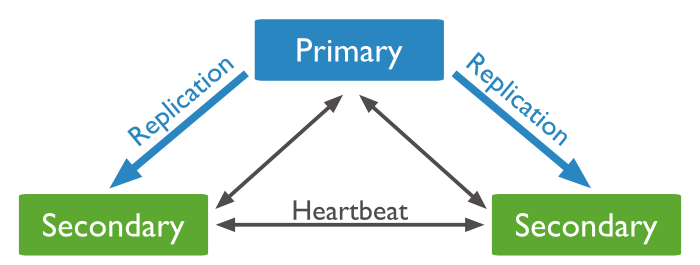
\includegraphics[width=0.7\textwidth]{img/mongodb-replica-set-primary-with-two-secondaries.png}
    \caption{MongoDB: Drie leden van een replicaset met 1 master en 2 slaves. \cite{mongodb-replicaset}}
    \label{fig:mongodb-replicaset}
\end{figure}

\begin{figure}[!htb]
	    \centering
    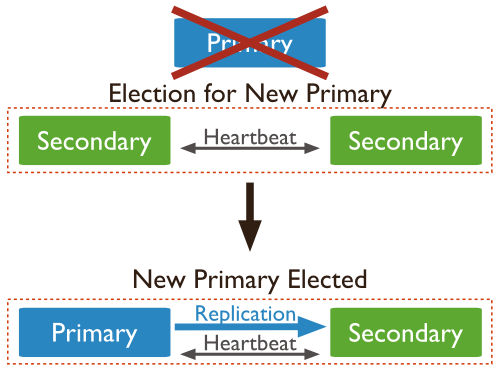
\includegraphics[width=0.7\textwidth]{img/mongodb-replica-set-trigger-election.png}
    \caption{MongoDB: Drie leden van een replicaset met 1 master en 2 slaves. \cite{mongodb-replicaset}}
    \label{fig:mongodb-replicaset-vote}
\end{figure}

\paragraph{} Vervolgens wordt met behulp van \textit{sharding} de data verdeeld over verschillende shards. In productie omgeving wordt aangeraden om een replicaset te nemen als shard maar het is ook mogelijk om een enkele node toe te voegen. 

Voor lees- en schrijfoperaties wordt er hier connectie gemaakt met mongos, dit zijn router nodes die de query naar de nodige shards stuurt. De configuratie van de shards wordt opgeslagen in 1 of 3 configuratie nodes (figuur \ref{fig:mongodb-shards}). 

\begin{figure}[!htb]
	    \centering
    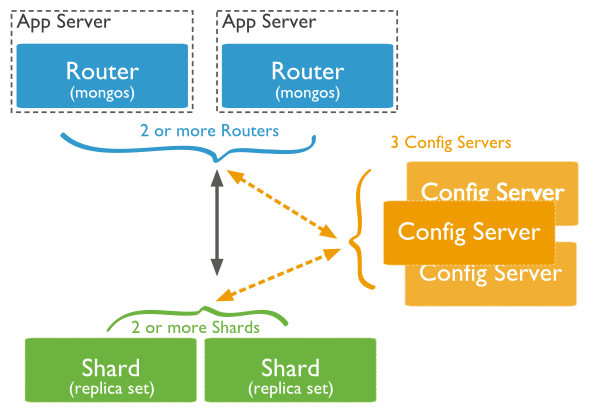
\includegraphics[width=\textwidth]{img/mongo-sharded-cluster-production-architecture.png}
    \caption{MongoDB: Een voorbeeld cluster voor productie met 2 mongos, 3 shards en 3 configuratie servers. \cite{mongodb-shard}}
    \label{fig:mongodb-shards}
\end{figure}

De data wordt verdeeld over de verschillende shards met een door de gebruiker gedefinieerde formule, dit kan door middel van hashing of door het opsplitsen van een waarde in verschillende domeinen. 

\paragraph{} De configuratie van MongoDB is opgesplitst in 2 delen, een configuratiebestand en met behulp van de shell. Als eerste stelt men een configuratiebestand op die aan de instantie basisinformatie meegeeft zoals op welke poort, waar de database op het bestandssysteem op te slaan en welk type de instantie is (enkele node, deel van replicaset, configuratie server of een mongos). 

Het opzetten van de replicasets en sharding verloopt via de shell, met behulp van een commando op een instantie die een deel is van de replicaset kan de replicaset opgezet worden. 
Sharding wordt opgezet door connectie te maken met een mongos en ook hier via commando shards toe te voegen, collecties aan te maken en collecties te verdelen onder shards.

Belangrijk bij sharding is dat bij het opstarten van een mongos al de verschillende configuratie servers meegegeven moeten worden, dit is de enige parameter die meegegeven moet worden in de configuratiebestanden die afhankelijk is van andere instanties. 

\subsection{Uitwerking}


\begin{figure}[!htb]
	    \centering
    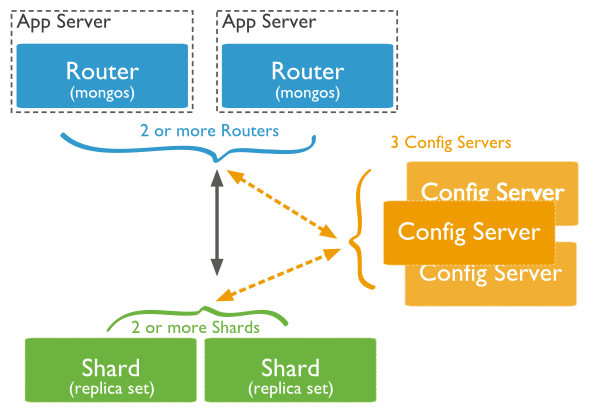
\includegraphics[width=\textwidth]{img/mongo-sharded-cluster-production-architecture.png}
    \caption{MongoDB: Een voorbeeld cluster voor productie met 2 mongos, 3 shards en 3 configuratie servers. \cite{mongodb-shard}}
    \label{fig:mongodb-shards}
\end{figure}
\subsection{Resultaat}

\chapter{Besluit}
\label{besluit}
De masterproeftekst wordt afgesloten met een hoofdstuk waarin alle
besluiten nog eens samengevat worden. Dit is ook de plaats voor suggesties
naar het verder gebruik van de resultaten, zowel industri"ele toepassingen
als verder onderzoek.

%%% Local Variables: 
%%% mode: latex
%%% TeX-master: "masterproef"
%%% End: 


% Indien er bijlagen zijn:
\appendixpage*          % indien gewenst
\appendix
%\chapter{De eerste bijlage}
\label{app:A}
In de bijlagen vindt men de data terug die nuttig kunnen zijn voor de
lezer, maar die niet essentieel zijn om het betoog in de normale tekst te
kunnen volgen. Voorbeelden hiervan zijn bronbestanden,
configuratie-informatie, langdradige wiskundige afleidingen, enz.

In een bijlage kunnen natuurlijk ook verdere onderverdelingen voorkomen,
evenals figuren en referenties\cite{h2g2}.

\section{Meer lorem}
\lipsum[50]

\subsection{Lorem 15--17}
\lipsum[15-17]

\subsection{Lorem 18--19}
\lipsum[18-19]

\section{Lorem 51}
\lipsum[51]

%%% Local Variables: 
%%% mode: latex
%%% TeX-master: "masterproef"
%%% End: 

% ... en zo verder tot
%\chapter{De laatste bijlage}
\label{app:n}
In de bijlagen vindt men de data terug die nuttig kunnen zijn voor de
lezer, maar die niet essentieel zijn om het betoog in de normale tekst te
kunnen volgen. Voorbeelden hiervan zijn bronbestanden,
configuratie-informatie, langdradige wiskundige afleidingen, enz.

\section{Lorem 20-24}
\lipsum[20-24]

\section{Lorem 25-27}
\lipsum[25-27]

%%% Local Variables: 
%%% mode: latex
%%% TeX-master: "masterproef"
%%% End: 


\backmatter
% Na de bijlagen plaatst men nog de bibliografie.
% Je kan de  standaard "abbrv" bibliografiestijl vervangen door een andere.
\printglossary

\printbibliography


\end{document}

%%% Local Variables: 
%%% mode: latex
%%% TeX-master: t
%%% End: 
